\section{Reducción de dimensionabilidad}
%Experimentamos con la técnica de selección univariada conocida como \textit{Ranking de atributos} para eliminar las palabras que no aportan información relevante
%para la clasificación. Esta técnica consiste en generar un ranking de atributos evaluando cada uno por separado para luego elegir los K mejores rankeados. \\
%En un primer intento tratamos de realizar la reducción utilizando la combinación de dos tipos de selecciones posibles, Ranking de atributos y PCA.
%Pero esto no fue posible ya que nos encontramos con incompatibilidades en las funciones de las librerías.
% Es por esto que decidimos experimentar unicamente con el selector \textit{KBest}, quedandonos con los primeros 100 del ranking.


Para una selección mas inteligente de los atributos quisimos experimentar con PCA. Pero 
esto no fue posible ya que nos encontramos con incompatibilidades en las funciones de las librerías. \\

Por este motivo solo experimentamos con la técnica de selección univariada conocida como 
\textbf{Ranking de Atributos} para eliminar las palabras que no aportan información relevante para la clasificación. Esta selección funciona mediante la selección de las mejores features en base a test estadísticos univariados en particular nosotros elegimos 
la métrica de scoring ANOVA F-value \\

Para determinar qué K o percentil nos quedamos, es decir, el límite a partir del cual consideramos que los atributos dejan de ser relevantes, habría que hacer una experimentación y análisis estadístico que van más allá del objetivo del trabajo práctico, aunque entendemos que es un factor importante en la selección de atributos. \\

Presentamos un histograma con los scores que dio la métrica f\_classif para los 50 atributos más relevantes en una instancia. 

\begin{center}
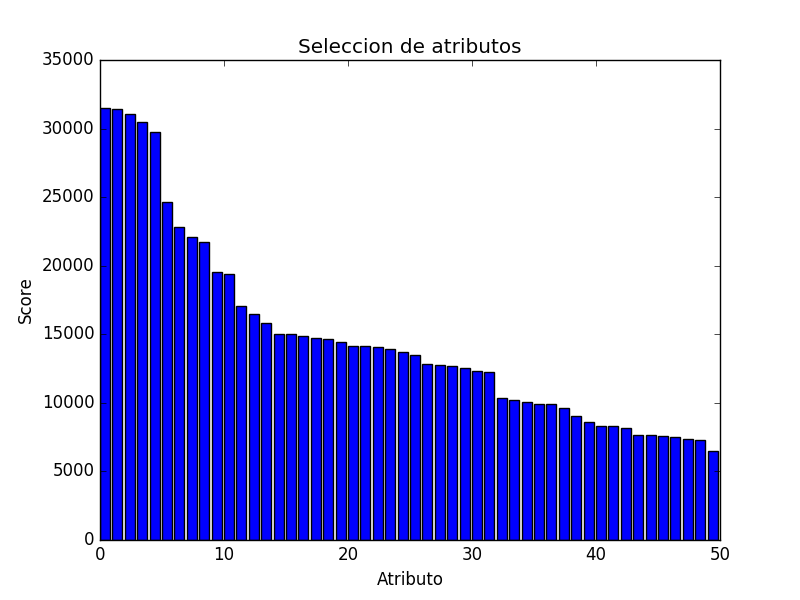
\includegraphics[height=8cm, width=10cm]{Seleccion_atributos.png}
\end{center}